\chapter{Implementacija i korisničko sučelje}
		
		
		\section{Korištene tehnologije i alati}
		
			\textbf{\textit{dio 2. revizije}}
			
			 \textit{Detaljno navesti sve tehnologije i alate koji su primijenjeni pri izradi dokumentacije i aplikacije. Ukratko ih opisati, te navesti njihovo značenje i mjesto primjene. Za svaki navedeni alat i tehnologiju je potrebno \textbf{navesti internet poveznicu} gdje se mogu preuzeti ili više saznati o njima}.
			
			
			\eject 
		
	
		\section{Ispitivanje programskog rješenja}
			
			\textbf{\textit{dio 2. revizije}}\\
			
			 \textit{U ovom poglavlju je potrebno opisati provedbu ispitivanja implementiranih funkcionalnosti na razini komponenti i na razini cijelog sustava s prikazom odabranih ispitnih slučajeva. Studenti trebaju ispitati temeljnu funkcionalnost i rubne uvjete.}
	
			
			\subsection{Ispitivanje komponenti}
			\textit{Potrebno je provesti ispitivanje jedinica (engl. unit testing) nad razredima koji implementiraju temeljne funkcionalnosti. Razraditi \textbf{minimalno 6 ispitnih slučajeva} u kojima će se ispitati redovni slučajevi, rubni uvjeti te izazivanje pogreške (engl. exception throwing). Poželjno je stvoriti i ispitni slučaj koji koristi funkcionalnosti koje nisu implementirane. Potrebno je priložiti izvorni kôd svih ispitnih slučajeva te prikaz rezultata izvođenja ispita u razvojnom okruženju (prolaz/pad ispita). }
			
			 

			\subsection{Ispitivanje sustava}
Ispitivanje sustava ostvareno je Selenium WebDriverom u Pythonu. Selenium WebDriver je alat za automatizaciju web preglednika. WebDriver koristi preglednikove vlastite mehanizme za kontrolu, čime osigurava visoku razinu realističnosti u testiranju, što ga čini ključnim alatom u razvoju softvera i osiguravanju kvalitete web aplikacija. Provedeni testovi s kodom priloženi su u nastavku.
\break

\begin{figure}[htp]
    \caption{prvi ispitni slučaj koji obrađuje ispravnu prijavu. Očekivani izlaz je uspješna prijava i preusmjeravanje.}
    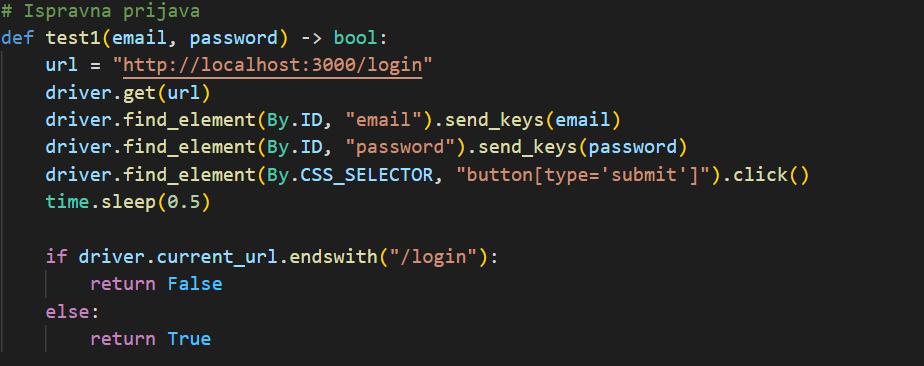
\includegraphics[scale=0.5]{dijagrami/test1.png}
    \centering
    
\end{figure}
\break

\begin{figure}[htp]
    \caption{drugi ispitni slučaj koji obrađuje neispravnu registraciju. Unosom maila u krivom formatu očekivani izlaz je neuspjela registracija.}
    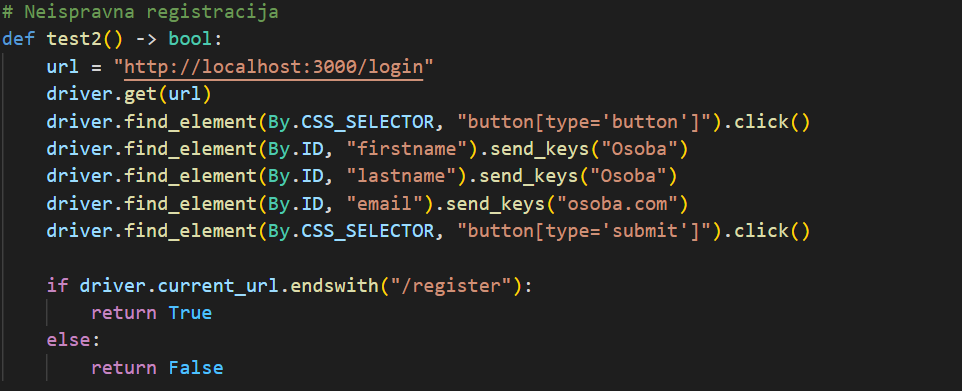
\includegraphics[scale=0.5]{dijagrami/test2.png}
    \centering
    
\end{figure}
\break

\begin{figure}[htp]
    \caption{treći ispitni slučaj koji obrađuje uspješnu promjenu lozinke. Preduvjet za promjenu lozinke je uspješna prijava u sustav kao student. Unosom podudarajućih lozinki očekivani izlaz je izmjena lozinke i preusmjeravanje.}
    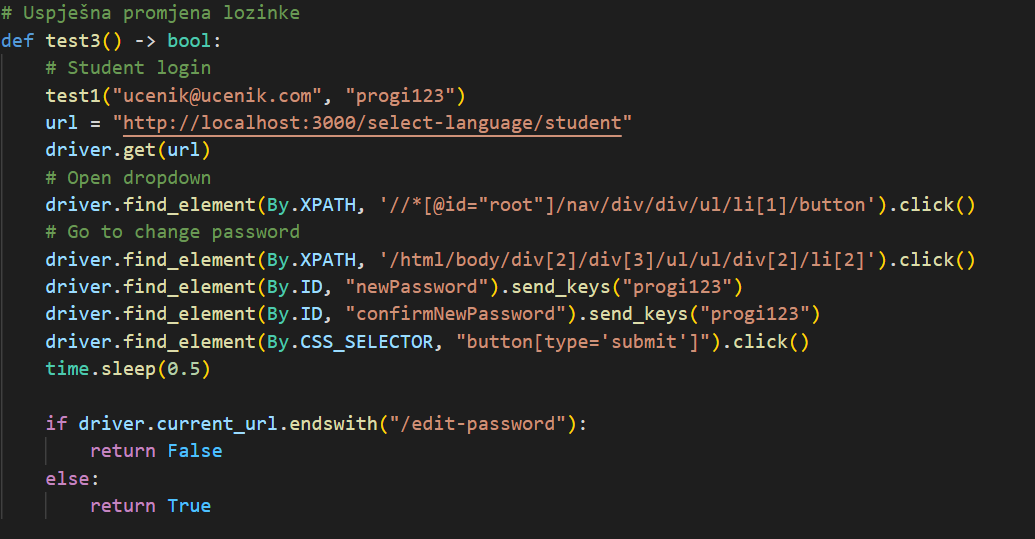
\includegraphics[scale=0.5]{dijagrami/test3.png}
    \centering
    
\end{figure}
\break

\begin{figure}[htp]
    \caption{četvrti ispitni slučaj koji obrađuje neispravno stvaranje admina. Preduvjet za stvaranje admina je uspješna prijava u sustav kao admin. Unosom nepodudarajućih lozinki u predložak, očekivani izlaz je neuspjela kreacija admina.}
    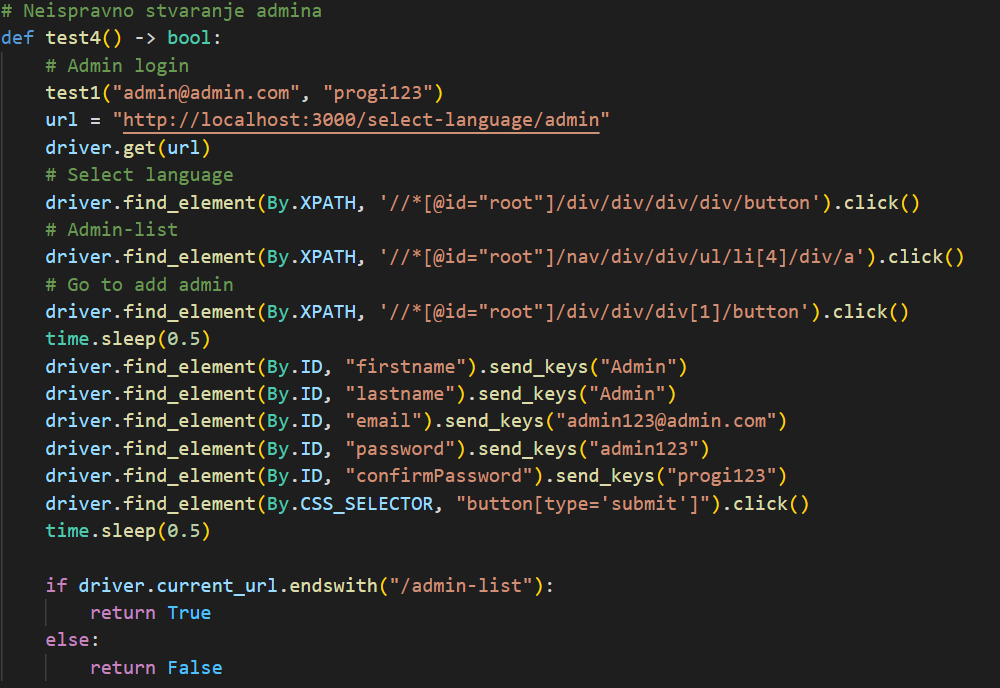
\includegraphics[scale=0.5]{dijagrami/test4.png}
    \centering
    
\end{figure}
\break

\begin{figure}[htp]
    \caption{peti ispitni slučaj koji obrađuje stvaranje rječnika s praznim imenom. Preduvjet za stvaranje rječnika je uspješna prijava u sustav kao admin. Bez unosa imena novog rječnika očekivani izlaz je nepromijenjeno stanje tablice rječnika u sustavu.}
    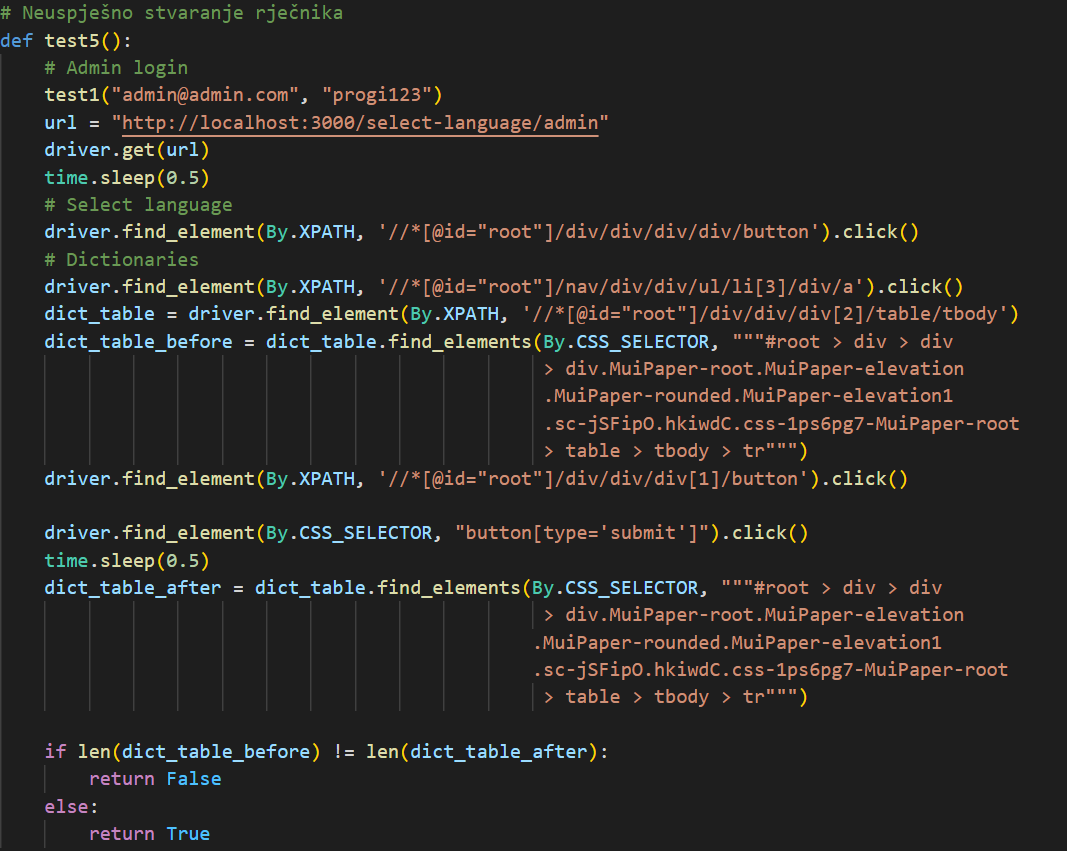
\includegraphics[scale=0.5]{dijagrami/test5.png}
    \centering
    
\end{figure}
\break

\begin{figure}[htp]
    \caption{terminal nakon pokretanja testova ispitivanja sustava.}
    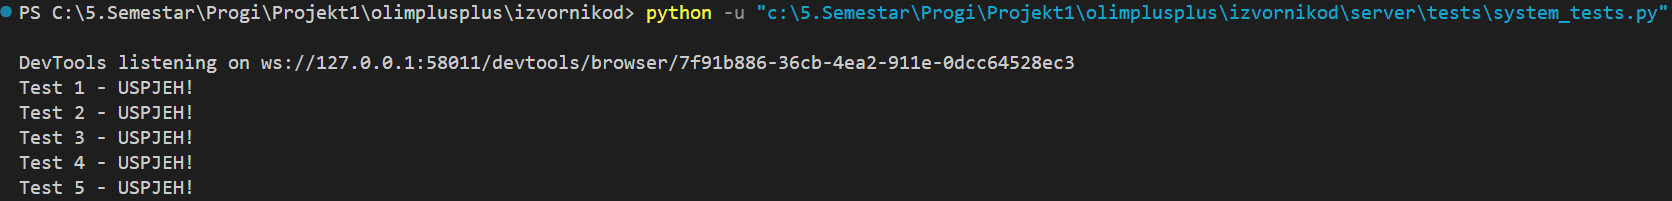
\includegraphics[scale=0.4]{dijagrami/terminal_screen.png}
    \centering
    
\end{figure}
\eject

		
		\section{Dijagram razmještaja}
			
		\begin{figure}[htp]
			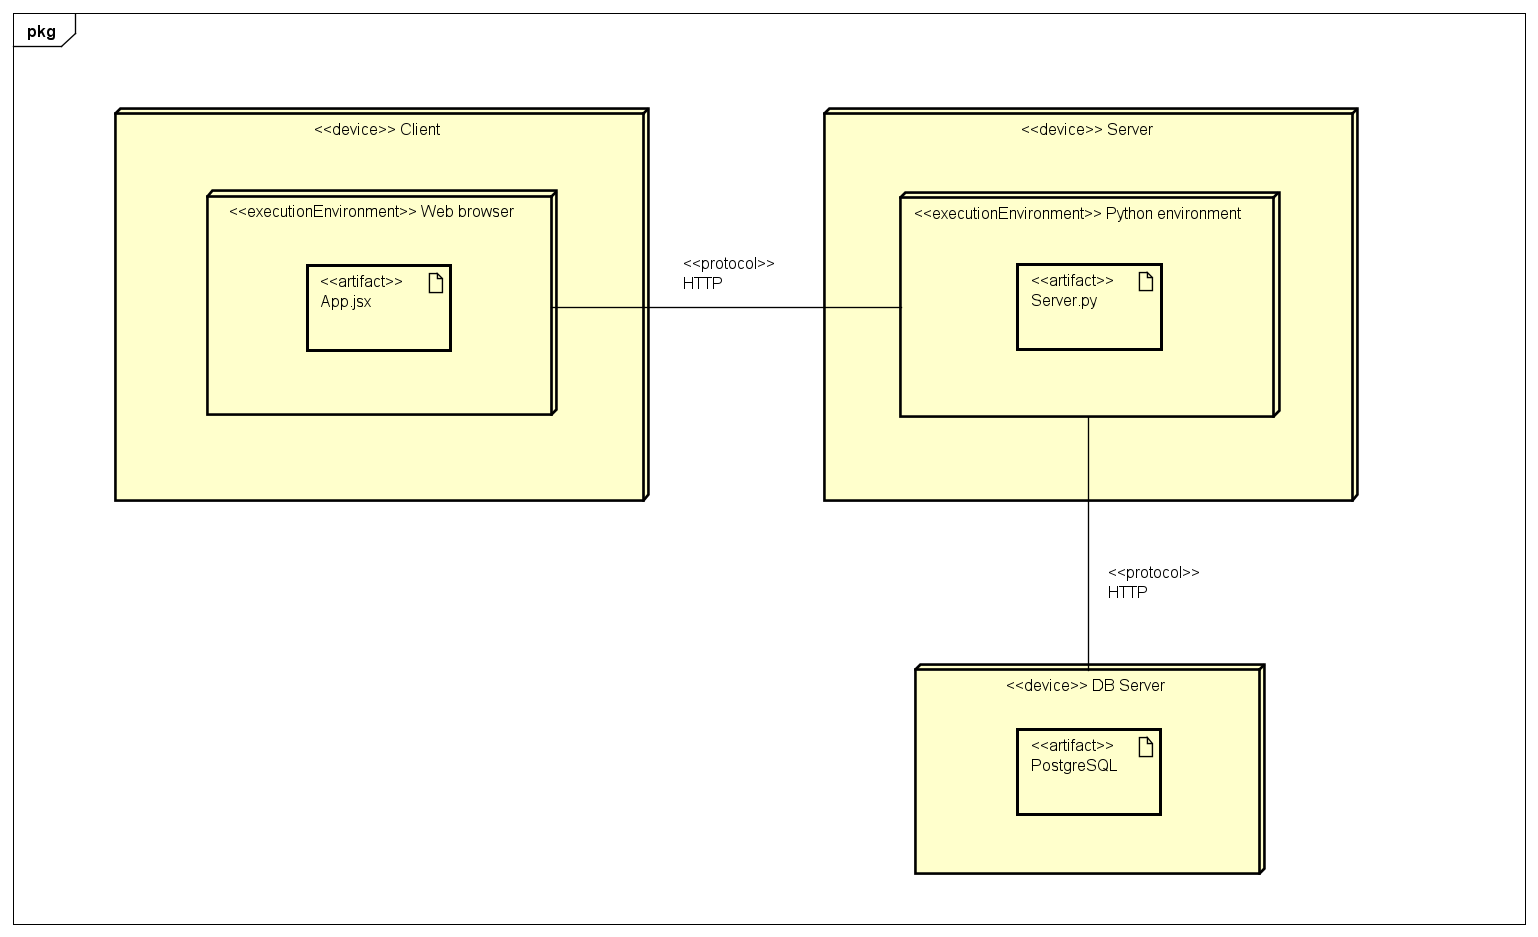
\includegraphics[scale=0.4]{dijagrami/DeploymentDiagram0.png}
			\centering
			\caption{Dijagram razmještaja}
		\end{figure}
		
		\section{Upute za puštanje u pogon}
		
			\textbf{\textit{dio 2. revizije}}\\
		
			 \textit{U ovom poglavlju potrebno je dati upute za puštanje u pogon (engl. deployment) ostvarene aplikacije. Na primjer, za web aplikacije, opisati postupak kojim se od izvornog kôda dolazi do potpuno postavljene baze podataka i poslužitelja koji odgovara na upite korisnika. Za mobilnu aplikaciju, postupak kojim se aplikacija izgradi, te postavi na neku od trgovina. Za stolnu (engl. desktop) aplikaciju, postupak kojim se aplikacija instalira na računalo. Ukoliko mobilne i stolne aplikacije komuniciraju s poslužiteljem i/ili bazom podataka, opisati i postupak njihovog postavljanja. Pri izradi uputa preporučuje se \textbf{naglasiti korake instalacije uporabom natuknica} te koristiti što je više moguće \textbf{slike ekrana} (engl. screenshots) kako bi upute bile jasne i jednostavne za slijediti.}
			
			
			 \textit{Dovršenu aplikaciju potrebno je pokrenuti na javno dostupnom poslužitelju. Studentima se preporuča korištenje neke od sljedećih besplatnih usluga: \href{https://aws.amazon.com/}{Amazon AWS}, \href{https://azure.microsoft.com/en-us/}{Microsoft Azure} ili \href{https://www.heroku.com/}{Heroku}. Mobilne aplikacije trebaju biti objavljene na F-Droid, Google Play ili Amazon App trgovini.}
			
			
			\eject 